\documentclass{report}
\usepackage{graphicx} % Required for inserting images
\usepackage[english]{babel}
\usepackage{amsthm}
\usepackage{amsmath}
\usepackage{amsfonts}
\usepackage{tikz}
\usetikzlibrary{matrix}
\usepackage[english]{babel}
\usepackage{mathtools}

\title{MMath project}
\author{Saxon Supple }
\date{January 2024}

\newtheorem{definition}{Definition}
\newtheorem{lemma}{Lemma}
\newtheorem{theorem}{Theorem}
\newtheorem{proposition}{Proposition}
\newtheorem{corollary}{Corollary}
\newtheorem{example}{Example}
\newtheorem{remark}{Remark}

\begin{document}

\maketitle

\section{Singular homology}
\begin{definition}
A \textbf{k-simplex} is the convex hull\\
$[v_0,...,v_k]:=\{\sum_{i=0}^k\lambda_iv_i:\lambda_i\in [0,1],\sum_{i=0}^k\lambda_i=1\}$\\
of $k+1$ linearly independent vectors $v_0,...,v_k\in\mathbb{R}^n$.\\
The \textbf{standard k-simplex} is\\$\Delta^k=[e_0,...,e_k]=\{(t_0,...,t_k)\in\mathbb{R}^k:t_i\geq 0, \sum_{i=0}^kt_i=1\}$\\
The vectors $v_0,...,v_k$ define a \textbf{framing} $F_{v_0,...,v_k}\colon\Delta^k\rightarrow [v_0,...,v_k],(t_i)\mapsto \sum_{i=0}^kt_iv_i$.
\end{definition}


\noindent For example $\Delta^0$ is a point, $\Delta^1$ a line segment, $\Delta^2$ a triangle and $\Delta^3$ a tetrahedron.

\begin{definition}
The \textbf{faces} of $[v_0,...,v_k]$ are the (k-1)-simplices $[v_0,...,\overset{\wedge}{v_i},...,v_k]$ where $\overset{\wedge}{v_i}$ means omit the entry $v_i$.
\end{definition}

\begin{definition}
Let $X$ be a topological space. A \textbf{singular k-simplex} in X is a continuous map $\sigma\colon\Delta^k\to X$. The \textbf{k-th chain group} of $X$ is the abelian group\\
$C_k(X):=\{\sum_{i=1}^kn_i\sigma_i:k\in\mathbb{N}_0,n_i\in\mathbb{Z},\sigma_i \text{ is a k-simplex}\}$ where the elements are called \textbf{k-chains}.
\end{definition}
\begin{remark}
$C_k(X)$ is an example of a \textbf{free abelian group}; that is, an abelian group whose elements are of the form $\sum_in_is_i$ where each $s_i$ belongs to some set $S$.
\end{remark}


\begin{definition}
The \textbf{boundary map} $\partial=\partial_k\colon C_k(X)\to C_{k-1}(X)$ is given by\\
$\partial\sigma=\sum_{i=0}^k(-1)^i\sigma\circ F_{e_0,...,\overset{\wedge}{e_i},...,e_k}\in C_{k-1}(X)$\\
on single simplices and extended linearly to all of $C_k(X)$.\\
A k-chain $c\in C_k(X)$ is a \textbf{k-cycle} if $\partial(c)=0$.
\end{definition}
\noindent Intuitively this definition means that the boundary map decomposes $\sigma$ into a sum of maps to its faces--or rather the images of faces of $\Delta^k$--taking into account orientation.


\begin{lemma}
$\partial\circ\partial\colon C_k(X)\to C_{k-2}(x)$ is zero.
\end{lemma}
\begin{proof}
Let $\sigma\in C_k(X)$.\\
$\partial\circ\partial (\sigma)=\partial(\sum_{i=0}^k(-1)^i\sigma\circ F_{e_0,...,\overset{\wedge}{e_i},...,e_k})$\\
$=\sum_{i=0}^k(-1)^i\partial\circ\sigma\circ F_{e_0,...,\overset{\wedge}{e_i},...,e_k}$ by linearity\\
$=\sum_{i=0}^k(\sum_{j<i}(-1)^{i+j}\sigma\circ F_{e_0,...,\overset{\wedge}{e_j},...,\overset{\wedge}{e_i},...,e_k} + \sum_{i<j}(-1)^{i+j-1}\sigma\circ F_{e_0,...,\overset{\wedge}{e_i},...,\overset{\wedge}{e_j},...,e_k})$ (since $e_j$ gets shifted forward one spot when $e_i$ is removed first)\\
$=\sum_{i=0}^k(\sum_{j<i}(-1)^{i+j}\sigma\circ F_{e_0,...,\overset{\wedge}{e_j},...,\overset{\wedge}{e_i},...,e_k} + \sum_{j<i}(-1)^{i+j-1}\sigma\circ F_{e_0,...,\overset{\wedge}{e_j},...,\overset{\wedge}{e_i},...,e_k})$
(interchanging $j$ with $i$ in the second term)\\
$=\sum_{i=0}^k(\sum_{j<i}((-1)^{i+j}+(-1)^{1+j-1})\sigma\circ F_{e_0,...,\overset{\wedge}{e_j},...,\overset{\wedge}{e_i},...,e_k})=0$
\end{proof}

\noindent A simple example of this fact is that the boundary of a ball is a sphere, which in turn has no boundary.\\
It also implies that $\text{im}(\partial:C_{k+1}(X)\rightarrow C_k(X))\in\text{ker}(\partial:C_{k}(X)\rightarrow C_{k-1}(X))$,
allowing the following to be well-defined.
\begin{definition}
The \textbf{singular homology} of $X$ is the collection of abelian groups
$H_k(X)=\frac{\text{ker}(\partial:C_{k}(x)\rightarrow C_{k-1}(X))}{\text{im}(\partial:C_{k+1}(x)\rightarrow C_k(X))}$
\end{definition}

\noindent The utility of the homology groups are that homotopy-equivalent spaces have isomorphic homology groups, thereby giving a way to prove that two topological spaces aren't homotopy-equivalent. To prove this, we must first construct a functor sending a continuous map between topological spaces to a homomorphism between their homology groups.\\

\noindent To give a more general result we shall allow the chain groups to have coefficients in any abelian group $G$ as opposed to merely $\mathbb{Z}$.
\begin{definition}
The k-th singular chain group with coefficients in an abelian group $G$ is $C_k(X;G):=\{\sum_{i=1}^kn_i\sigma_i:k\in\mathbb{N}_0,n_i\in G,\sigma_i \text{ is a k-simplex}\}$ The boundary map $\partial\colon C_k(X;G)\to C_{k-1}(X;G)$ and k-th homology group with coefficients in $G$, $H_k(X;G)$, are then defined as above while replacing $\mathbb{Z}$ with $G$.
\end{definition}

\noindent Let $f\colon X\to Y$ be a continuous map between topological spaces. Given a k-simplex $\sigma\colon\Delta^k\to X$ in $X$, $f\circ\sigma$ is a k-simplex in $Y$. This gives rise to a homomorphism $f_\#\colon C_k(X;G)\to C_k(Y;G):\sum_{i=0}^kn_i\sigma_i\mapsto\sum_{i=0}^kn_if\circ\sigma_i$.
\begin{definition}
This induces a \textbf{push-forward homomorphism} $f_*\colon H_k(X;G)\to H_k(Y;G)$ sending $[c]$ to $[f_\#(c)]$.
\end{definition}
\noindent To show that this is well-defined, note that $\partial f_\#=f_\#\partial$ (in other words $f_\#$ is a chain map) and so $f_\#$ maps closed chains to closed chains. Furthermore suppose $[a-b]=[0]$. Then there exists a $\sigma\in C_{k+1}(X;G)$ such that $a-b=\partial\sigma\implies f_\#(a-b)=f_\#\partial\sigma=\partial f_\#\sigma\implies [f_\#(a)-f_\#(b)]=[0]=f_*([a])-f_*([b])$ as required.

\noindent This argument applies more generally to show that all chain maps induce a well-defined map on homology groups.

\begin{proposition}
The push-forward is a functor.
\end{proposition}
\begin{proof}
Let $X$, $Y$ and $Z$ be topological spaces.
Clearly $\text{id}_{X*}=\text{id}_{H_k(X;G)}$.\\
Now let $f\colon Y\to Z$ and $g\colon X\to X$ be continuous maps. Given $[c]=[\sum_{i=0}^kn_i\sigma_i]\in H_k(X;G)$, $(f\circ g)_*([c])=[\sum_{i=0}^kn_if\circ g(\sigma_i)]=f_*([\sum_{i=0}^kn_ig(\sigma_i)])=f_*\circ g_*([c])$ so $(f\circ g)_*=f_*\circ g_*$.
\end{proof}

\noindent This then implies the standard results from category theory such as the push-forward sending commutative diagrams to commutative diagrams and homeomorphisms to group isomorphisms.

\begin{lemma}
If $f,g\colon X\to Y$ are homotopic continuous maps between topological spaces then $f_*=g_*\colon H_k(X)\to H_k(Y)$
\end{lemma}
\begin{proof}
Let $F\colon X\times I\to Y$ be a homotopy from $f$ to $g$. Given a singular n-simplex $\sigma\colon\Delta^n\to X$ we can define $\sigma\times\text{id}\colon\Delta^n\times I\to X\times I$ and $F_\#(\sigma\times\text{id})\colon\Delta^n\times I\to Y$. We now decompose $\Delta^n\times I$ as the union of $n+1$-simplices. To do this write $\Delta^n\times I$ as $[a_0,...,a_n,b_0,...,b_n]$ where $a_i=(e_i,0)$ and $b_i=(e_i,1)$. Then $\Delta^n\times I$ is the union of the $n+1$-simplices $\alpha_i=[a_0,...,a_i,b_i,...,b_n]$. Now define the "prism map" $P\colon C_n(X)\to C_{n+1}(Y)$ by $P(\sigma)=\sum_i(-1)^iF\circ(\sigma\times\text{id})|_{\alpha_i}$. $\partial P(\sigma)=\sum_i(-1)^i[\sum_{j\leq i}(-1)^jF\circ(\sigma\times\text{id})|_{[a_0,...,\overset{\wedge}{a_j},...,a_i,b_i,...,b_n]}+\sum_{j> i}(-1)^{(j+1)}F\circ(\sigma\times\text{id})|_{[a_0,...,a_i,b_i,...,\overset{\wedge}{b_j},...,b_n]}]$. The sum of terms with $i=j$ is $F\circ(\sigma\times\text{id})|_{[\overset{\wedge}{a_0},b_0,...,b_n]}-F\circ(\sigma\times\text{id})|_{[a_0,\overset{\wedge}{b_0},b_1,...,b_n]}+F\circ(\sigma\times\text{id})|_{[a_0,\overset{\wedge}{a_1},b_1,...,b_n]}-F\circ(\sigma\times\text{id})|_{[a_0,a_1,\overset{\wedge}{b_1},...,b_n]}+...+F\circ(\sigma\times\text{id})|_{[a_0,...,\overset{\wedge}{a_n},b_n]}-F\circ(\sigma\times\text{id})|_{[a_0,...,a_n,\overset{\wedge}{b_n}]}=F\circ(\sigma\times\text{id})|_{[\overset{\wedge}{a_0},b_0,...,b_n]}-F\circ(\sigma\times\text{id})|_{[a_0,...,a_n,\overset{\wedge}{b_n}]}=F\circ(\sigma\times\text{id})|_{[b_0,...,b_n]}-F\circ(\sigma\times\text{id})|_{[a_0,...,a_n]}$ as a telescoping sum which is then $=g\circ\sigma-f\circ\sigma=(g_\#-f_\#)(\sigma)$. The terms with $i\neq j$ can be identified with $-P(\partial\sigma)$ so that $\partial P\sigma=-P(\partial\sigma)+g_\#(\sigma)-f_\#(\sigma)\implies\partial P + P\partial=g_\#-f_\#$. $\partial(\partial P + P\partial)=\partial P\partial=(\partial P + P\partial)\partial$ so $(\partial P + P\partial)$ is a chain map inducing a homomorphism on homology groups. Furthermore given a cycle $\sigma$ we have $(\partial P + P\partial)(\sigma)=\partial P(\sigma) + P\partial(\sigma)=\partial P(\sigma)$ so $\partial P(\sigma)$ sends cycles to boundaries thereby inducing the zero map on homology groups. Thus $g_*-f_*=0$ or $f_*=g_*$.
\end{proof}


\noindent We are now ready to prove that homology is a topological invariant.
\begin{proposition}
If $X$ and $Y$ are homotopy-equivalent then $H_k(X;G)\cong H_k(Y;G)$
\end{proposition}
\begin{proof}
We have continuous maps $f\colon X\to Y$ and $g\colon Y\to X$ such that $g\circ f\simeq\text{id}_X$ and $f\circ g\simeq\text{id}_Y$ giving $g_*\circ f_*=\text{id}_{H_k(X;G)}$ and $f_*\circ g_*=\text{id}_{H_k(Y;G)}$. Thus $f_*$ has a left and right inverse so is a bijection so a group isomorphism.
\end{proof}

\begin{lemma}
If $X$ is path-connected then $H_0(X)=\mathbb{Z}$.
\end{lemma}
\begin{proof}
A singular 0-simplex is a map from a point to a point $x\in X$. let $c=\sum n_i\sigma_i$ be a 0-chain. $\partial c=0$ so $\text{ker}(\partial:C_{0}(x)\rightarrow C_{-1}(X))=C_0(X)$ giving $H_0(X)=\frac{C_0(X)}{\partial C_1(X)}$. Let $x,y\in X$ and let $\sigma_x$ and $\sigma_y$ be their corresponding simplicial 0-simplices. $X$ is path-connected so there exists a simplicial 1-simplex $\sigma$ with $\partial\sigma=\sigma_x-\sigma_y$. Define $f\colon C_0(X)\to\mathbb{Z}:\sum n_ix_i\mapsto\sum n_i$. Clearly $\partial C_1(X)\in \text{ker}f$. Let $z=\sum_{i=0}^ka_i\sigma_i\in\text{ker}f$. Express $a_i\sigma_i$ as $\sum_{j=1}^{|a_i|}a_{ij}\sigma_i$ where $a_{ij}$ is either all $1$ or all $-1$. Thus $z=\sum_{j=1}^rb_j\tau_j$ where $\tau_j\in\{\sigma_0,...,\sigma_k\}$ and $b_j=\pm1$. $|\{j:b_j=1\}|=|\{j:b_j=-1\}|$ so $r$ is even and we can express $z$ as a sum of terms of the form $(\sigma_\alpha - \sigma_\beta)\in\partial C_1(X)$, giving $\text{ker}f\in\partial C_1(X)$. Thus $\text{ker}f\in\partial C_1(X)$. $f$ is surjective so the result follows by the first isomorphism theorem.
\end{proof}

\begin{lemma}
$H_k(\{\text{pt}\})=\begin{cases}
       \mathbb{Z} &\quad\text{if }k=0 \\
       0 &\quad\text{otherwise} \\ 
     \end{cases}$
\end{lemma}
\begin{proof}
There is only one k-simplex $\sigma_k\colon\Delta^k\rightarrow \{\text{pt}\}$, the constant map. Thus $C_k(\{\text{pt}\})=\{n\sigma_k:n\in\mathbb{Z}\}=\mathbb{Z}$.
Also $\partial_k(n\sigma_k)=\sum_{i=0}^k(-1)^i n\sigma_{k-1}$ which is zero if $k$ is odd and $n\sigma_{k-1}$ if $k$ is even. Thus the induced map on the coefficients of the boundary is $0$ if $k$ is odd and id if $k$ is even. The Homology groups will then be $\frac{\mathbb{Z}}{\mathbb{Z}}=0$ or $\frac{\{0\}}{\{0\}}=0$, except for $H_0$ which is $\mathbb{Z}$ since $\{\text{pt}\}$ is path-connected.
\end{proof}


\begin{definition}
The \textbf{commutator subgroup} of a group $G$, denoted $[G,G]$, is the subgroup generated by all elements, called $commutators$, of the form $ab(ba)^{-1}$ for any $a$ and $b$ in $G$.
\end{definition}

\begin{lemma}
$[G,G]$ is a normal subgroup.
\end{lemma}
\begin{proof}
Let $g\in G,aba^{-1}b^{-1}\in [G,G]$.\\
$g^{-1}(aba^{-1}b^{-1})g=g^{-1}agg^{-1}bgg^{-1}a^{-1}gg^{-1}b^{-1}g$\\
$=(g^{-1}ag)(g^{-1}bg)(g^{-1}a^{-1}g)(g^{-1}b^{-1}g)$\\
$=(g^{-1}ag)(g^{-1}bg)(g^{-1}ag)^{-1}(g^{-1}bg)^{-1}\in[G,G]$.
\end{proof}
\begin{definition}
The \textbf{abelianization} $G^{\text{ab}}$ of a group $G$ is $G/[G,G]$.
\end{definition}
\noindent As the name suggests, $G^{\text{ab}}$ is abelian since we quotiented out by the relation that $ab=ba$ for all $a,b\in G$. If $G$ is already abelian then $[G,G]$ is trivial so $G^{\text{ab}}=G$.

\begin{lemma}
Given groups $G$ and $H$, where $H$ is abelian, and a group homomorphism $h\colon G\to H$, the induced homomorphism $h'\colon G^{\text{ab}}\to H:[x]\mapsto h(x)$ is well-defined.
\end{lemma}
\begin{proof}
Let $[x]=[y]\in G^{\text{ab}}$ so that $x=y\prod_ia_ib_ia_i^{-1}b_i^{-1}$ for $a_i,b_i\in G$.
Then $h'([x])=h(y\prod_ia_ib_ia_i^{-1}b_i^{-1})=h(y)\prod_ih(a_i)h(b_i)h(a_i)^{-1}h(b_i)^{-1}=h(y)=h'([y])$ since $H$ is abelian.
\end{proof}

\begin{lemma}
Let $G$ be a group. If $w$ is a word in $G$ such that for any $g\in G$ the exponents of $g$ in $w$ sum to zero then $w\in[G,G]$ 
\end{lemma}
\begin{proof}
Consider the quotient map $\pi\colon G\to G/[G,G]:g\mapsto[g]$.
$G/[G,G]$ is abelian so the letters in $[w]$ can be reordered such that $[w]=\sum n_i[a_i]=0$ implying $w\in\text{ker }\pi=[G,G]$. 
\end{proof}

\begin{theorem}
(Hurewicz). If $X$ is path-connected then $H_1(X)\cong\pi_1(X)^{\text{ab}}$.
\end{theorem}
\begin{proof}
First note that an element of $\pi_1(X,x_0)$ is of the form $[\gamma]$ for $\gamma\colon [0,1]\to X$ a loop based at $x_0$. $[0,1]=\Delta^1$ so $\gamma$ is a 1-simplex and $\partial(\gamma)=x_0-x_0$ making $\gamma$ closed.
We can then define $h\colon\pi_1(X,x_0)\to H_1(X)$ sending an element $[\gamma]\in\pi_1(X,x_0)$ to $[c_\gamma]\in H_1(X)$ where $c_\gamma$ is $\gamma$ as an element of $C_1(X)$. To show that $h$ is well-defined let $[a]=[b]\in\pi_1(X,x_0)$ and let $F\colon [0,1]^2\to X$ be a based-homotopy from $a$ to $b$. Dividing $[0,1]^2$ into two triangles and parametrising each by $\Delta^2$ allows F to be expressed as $c_F\in C_2(X)$ with $\partial c_F=c_a-c_b\implies [c_a]=[c_b]$ as required.

\noindent \textbf{Next we show that $h$ is a homomorphism.}\\
Let $[f],[g]\in\pi_1(X,x_0)$ and Define a singular 2-simplex $\sigma\colon\Delta^2\to X$ where $\sigma_{|[e_0,e_1]}=f$, $\sigma_{|[e_1,e_2]}=g$ and $\sigma_{|[e_0,e_2]}=f\cdot g$. Then $\partial(\sigma)=g-f\cdot g+f$ so $h([f][g])=h([f])+h([g])$ making $h$ a homomorphism.

\noindent \textbf{We now show that $h$ is surjective.}\\
For the sake of lucidity we will write $[\gamma]$ for $h([\gamma])$ instead of $[c_\gamma]$\\
Let $[\lambda]\in H_1(X)$ where $\lambda=\sum_{i=0}^k n_i\sigma_i$.
$\partial (\lambda)=0=\sum_{i=0}^k n_i(\sigma_i(1)-\sigma_i(0))$.\\
Let $\Lambda=\{\sigma_i(0)\}\cup\{\sigma_i(1)\}$ be the collection of end-points of the $\sigma_i$s.
For each $p\in\Lambda$ pick a path $\beta_p\colon [0,1]\to X$ from $x_0$ to $p$ (which is possible because $X$ is path-connected). Then $\sum_{i=0}^k n_i(\sigma_i(1)-\sigma_i(0))=\sum m_pp=0$ where $m_p$ is the sum of the coefficients of $p$ in the sum. This implies that $m_p=0 \forall p$. Now consider the loop $\eta_i=\beta_{\sigma_i(0)}\cdot\sigma_i\cdot\beta_{\sigma_i(1)}^{-1}$ based at $x_0$. Then $h([\eta_0^{n_0}\cdot\eta_1^{n_1}...\cdot\eta_k^{n_k}])=[n_0\eta_0+...+n_k\eta_k]=[\sum_{i=0}^kn_i(\beta_{\sigma_i(0)}+\sigma_i-\beta_{\sigma_i(1)})]=[\sum_{i=0}^kn_i\sigma_i+\sum_{i=0}^kn_i(\beta_{\sigma_i(0)}-\beta_{\sigma_i(1)})]=[\sum_{i=0}^kn_i\sigma_i-\sum m_p\beta_p]=[\sum_{i=0}^kn_i\sigma_i]=[\lambda]$ since $m_p=0$.\\
\noindent\textbf{We now find the kernel}\\
Let $[\gamma]\in\pi_1(X,x_0)$ such that $h([\gamma])=[0]$.
Then $\gamma$ is exact so there exists a finite sum of singular 2-simplices $\sum_{i=0}^kn_i\sigma_i$ such that $\gamma=\partial(\sum_{i=0}^kn_i\sigma_i)=\sum_{i=0}^kn_i\partial(\sigma_i)=\sum_{i=0}^kn_i(\lambda_i+\mu_i+\nu_i)$. Let $\Lambda=\{\lambda_i\}\cup\{\mu_i\}\cup\{\nu_i\}$ and for each end-point $p$ of a singular 1-simplex in $\Lambda$ let $\beta_p$ be a path from $x_0$ to $p$. For each $\theta\in\Lambda$ let $m_\theta$ be the sum of coefficients of $\theta$ in $\sum_{i=0}^kn_i(\lambda_i+\mu_i+\nu_i)$. This sum is equal to $\gamma$ thus $m_\theta$ is $1$ if $\theta=\gamma$ and $0$ otherwise. For each singular 2-simplex $\sigma_i$ the loops $\beta_{\lambda_i(0)}\cdot\lambda_i\cdot\beta_{\lambda_i(1)}^{-1}$, $\beta_{\mu_i(0)}\cdot\mu_i\cdot\beta_{\mu_i(1)}^{-1}$ and $\beta_{\nu_i(0)}\cdot\nu_i\cdot\beta_{\nu_i(1)}^{-1}$ have null-homotopic concatenations. Let $\eta_i=\beta_{\partial\sigma_i(0)}\cdot\partial\sigma_i\cdot\beta_{\partial\sigma_i(1)}^{-1}$. Then $h([\eta_0^{n_0}\cdot...\cdot\eta_k^{n_k}\cdot\gamma^{-1}])=h([\gamma])h([\gamma^{-1}])=[\gamma^{-1}]$. Now write each $[\eta_i]$ as $[\beta_{\lambda_i(0)}\cdot\lambda_i\cdot\beta_{\lambda_i(1)}^{-1}][\beta_{\mu_i(0)}\cdot\mu_i\cdot\beta_{\mu_i(1)}^{-1}][\beta_{\nu_i(0)}\cdot\nu_i\cdot\beta_{\nu_i(1)}^{-1}]$. Then for each $\theta\in\Lambda$ we have that the sum of exponents of $[\beta_{\theta(0)}\cdot\theta\cdot\beta_{\theta(1)}^{-1}]$ is $m_\theta$ The exponents of each $[\beta_{\theta(0)}\cdot\theta\cdot\beta_{\theta(1)}^{-1}]$ in $[\eta_0^{n_0}\cdot...\cdot\eta_k^{n_k}\cdot\gamma^{-1}]$ is then 0 so by the above lemma $[\gamma^{-1}]\in[\pi_1(X,x_0),\pi_1(X,x_0)]$ meaning $[\gamma]$ is as well. Thus $\text{ker }h\subseteq [\pi_1(X,x_0),\pi_1(X,x_0)]$. We also have that $[\pi_1(X,x_0),\pi_1(X,x_0)]\subseteq \text{ker }h$ since $H_1(X)$ is abelian so $\text{ker }h=[\pi_1(X,x_0),\pi_1(X,x_0)]$. The result then follows by the first isomorphism theorem.
\end{proof}

\begin{corollary}
$H_1(S^n)=$$\begin{cases}
       \mathbb{Z} &\quad\text{if }n=1 \\
       0 &\quad\text{otherwise} \\ 
     \end{cases}$\\
$H_1(T^2)=\mathbb{Z}^2$\\
$H_1(\mathbb{R}P^n)=$$\begin{cases}
       \mathbb{Z} &\quad\text{if }n=1 \\
       \mathbb{Z}_2 &\quad\text{otherwise} \\ 
     \end{cases}$\\
$H_1(K)=\mathbb{Z}\bigoplus\mathbb{Z}_2$
\end{corollary}

\section{Cohomology}

\begin{definition}
Let $R$ be a commutative ring with a unit. An \textbf{R-module} $M$ is an abelian group with a map $f\colon R\times M\to M$ such that if $f(r,m)$ is denoted by $rm$ then $(r_1r_2)m=r_1(r_2m)$ and $1m=m$. We usually abbreviate R-modules to modules.
\end{definition}
\begin{remark}
More specifically we defined a \textbf{left R-module}. If $f$ instead had domain $M\times R$ then $M$ would be a \textbf{right R-module}.
\end{remark}

\begin{definition}
Let $M$ and $N$ be R-modules. An \textbf{R-module homomorphism} $f\colon M\to N$ is a homomorphism of abelian groups such that $f(rm)=rf(m)$ 
\end{definition}

\begin{example}
An abelian group $G$ is a $\mathbb{Z}$-module given by $ng=$$\begin{cases}
       \sum_{i=1}^ng &\quad\text{if }n>0 \\
       0 &\quad\text{if }n=0 \\
       -\sum_{i=1}^{-n}g &\quad\text{if }n<0 \\
     \end{cases}$\\
\end{example}

\begin{definition}
Let $A$ and $B$ be R-modules. Their \textbf{direct sum} $A\bigoplus B$ is the module $A\times B$ under component-wise operations i.e. $(a_1,b_1)+(a_2,b_2)=(a_1+a_2,b_1+b_2)$ and $r(a,b)=(ra,rb)$. This can be extended to any finite collection of R-modules.
\end{definition}

\begin{definition}
A bilinear map $h\colon M\times N\to P$ is a map such that $h(m_1+m_2,n)=h(m_1,n)+h(m_2,n)$, $h(m,n_1+n_2)=h(m,n_1)+h(m,n_2)$ and $h(rm,n)=h(m,rn)$ for $r\in R$.
\end{definition}

\begin{definition}
Given modules M and N, we define the module $R^{M\times N}$ to be $\{\sum_{i=0}^kr_i(m_i,n_i):r_i\in R,(m_i,n_i)\in M\times N\}$.
\end{definition}

\begin{definition}
Given a module M, we say that $H\subseteq M$ is a \textbf{submodule} if $rh\in H\forall r\in R,h\in H$ and $H$ is itself a module after inheriting the addition and multiplication maps of $M$.
\end{definition}

\begin{definition}
Given a module $M$ and submodule $N$, the \textbf{quotient R-module of M by N} is the quotient group $M/N$ with multiplication given by $r(a+N)=ra+N\forall r\in R,a+N\in M/N$.
\end{definition}

\begin{definition}
Let $M$ and $N$ be modules. Let $I$ denote the submodule of $M\times N$ generated by the set of elements of the form $(\lambda m_1+m_2,n)-\lambda(m_1,n)-(m_2,n)$, $(m,\lambda n_1+n_2)-\lambda(m,n_1)-(m,n_2)$ for $m,m_1,m_2\in M$, $n,n_1,n_2\in N$ and $\lambda\in R$. Then the \textbf{tensor product} of $M$ and $N$ is $M\bigotimes_R N=R^{M\times N}/I$ whose elements are represented as $m\otimes n$ for $m\in M$, $n\in N$.
\end{definition}

\noindent This gives rise to the relations\\ $(m_1+m_2)\otimes n=m_1\otimes n+m_2\otimes n$,\\
$m\otimes(n_1+n_2)=m\otimes n_1+m\otimes n_2$ and\\
$(rm)\otimes n=m\otimes (rn)=r(m\otimes n)$ for $r\in R$.

\begin{example}
If $p$ and $q$ are coprime then $\mathbb{Z}_p\bigotimes_\mathbb{Z}\mathbb{Z}_q=0$ since there exist $m,n\in\mathbb{Z}$ such that $mp+nq=1$ (Bezout's lemma) so $a\otimes b=(mp+nq)a\otimes b=(mpa)\otimes b + a\otimes(nqb)=0\forall a\otimes b\in\mathbb{Z}_p\bigotimes_\mathbb{Z}\mathbb{Z}_q$.
\end{example}
\begin{example}
$C_k(X;G)=C_k(X)\bigotimes_\mathbb{Z}G$.
\end{example}

\begin{example}
$\mathbb{Z}_m\bigotimes\mathbb{Z}_n=\mathbb{Z}_{gcd(m,n)}$.
\end{example}
\begin{proof}
We have the first isomorphism for modules that given a module homomorphism $f:M\to N$, $M/\text{ker }f\cong\text{im }f$ (the proof is analogous to the cases for groups, rings and vector spaces).
So, define a module homomorphism $g\colon\mathbb{Z}\to\mathbb{Z}_m\bigotimes\mathbb{Z}_n:z\mapsto z(1\otimes 1)$. $g$ is surjective so $\text{im }g=\mathbb{Z}_m\bigotimes\mathbb{Z}_n$. Clearly $<\text{gcd}(m,n)>\subseteq\text{ker }g$. Now let $x\notin <\text{gcd}(m,n)>$. Then $x=s\text{gcd}(m,n)+k$ with $0<k<\text{gcd}(m,n)$ by division with remainder. $g(x)=s\text{gcd}(m,n)(1\otimes 1)+g(k)=k(1\otimes 1)\neq 0\implies x\notin\text{ker }g$ so $x\in\text{ker }g\implies x\in<\text{gcd}(m,n)>$ giving $<\text{gcd}(m,n)>=\text{ker }g$.
\end{proof}


\begin{definition}
Let M and N be modules over a ring R. The set of all module homomorphisms from M to N is denoted by $\text{Hom}_R(M,N)$. It is an abelian group under pointwise addition and a module if R is commutative.
\end{definition}

\begin{definition}
Let $X$ be a topological space and let $G$ be an abelian group. The \textbf{kth cochain group with coefficients in G} is $C^k(X;G)=Hom(C_k(X),G)$. 
\end{definition}

\begin{definition}
We define $d\colon C^k(X;G)\to C^{k+1}(X;G)$ to be the dual of $\partial$ in the sense that if $\phi\in C^k(X;G)$ and $c\in C_{k+1}(X)$ then $(d\phi)(c)=\phi(\partial c)\in G$
\end{definition}

\noindent In particular, $(d\circ d\phi)(c)=(d\phi)(\partial c)=\phi(\partial\circ\partial c)=\phi(0)=0$ so $d^2=0$.

\begin{definition}
The \textbf{kth cohomology group with coefficients in $G$} is $H^k(X;G)=\frac{\text{ker}(d\colon C^k(X;G)\to C^{k+1}(X;G))}{\text{im}(d\colon C^{k-1}(X;G)\to C^k(X;G))}$. When G is $\mathbb{Z}$ we abbreviate it to $H^k(X)$ and call it simply the \textbf{kth cohomology group}.
\end{definition}

\begin{definition}
Let $f\colon X\to Y$ be a continuous map between topological spaces and $G$ be an abelian group. We have a homomorphism $f^\#\colon C^k(Y;G)\to C^k(X;G):A\mapsto f^\# A$ given by $f^\# A(c)=A(f_\#(c))$. This in turn induces the \textbf{pullback homomorphism} $f^*\colon H^k(Y;G)\to H^k(X;G):[A]\mapsto [f^\# A]$.
\end{definition}
\noindent $df^\# A(c)=f^\# A(\partial c)=f^\# dA(c)$ so $df^\#=f^\# d$. Thus $f^\#$ is a chain map so $f^*$ is well-defined.

\begin{lemma}
There is a well-defined mapping $H^k(X;G)\times H_k(X)\to G$ given by $([\phi],[c])=\phi(c)$.
\end{lemma}
\begin{proof}
Let $[\phi]=[\psi]$ so that $\phi-\psi=d\rho$ for some $\rho\in C^{k-1}(X;G)$. Then $(\phi-\psi)(c)=d\rho(c)=\rho(\partial c)=0$ since $c\in\text{ker }\partial$. Thus $\phi(c)=\psi(c)$.
Now let $[a]=[b]$ so that $a=b+\partial e$ for some $e\in C_{k+1}(X)$. $\phi(a)=\phi(b+\partial e)=\phi(b)+\phi(\partial e)=\phi(b)+d\phi(e)=\phi(b)$ since $\phi\in\text{ker }d$.
\end{proof}

\noindent This then give that $f^*$ is dual to $f_*$ in the sense that $f^*[A]([c])=[A](f_*([c]))$ for $[A]\in H^k(Y;G)$ and $[c]\in H_k(X)$.

\begin{proposition}
Pullback is a contravariant functor.
\end{proposition}
\begin{proof}
Let $X$, $Y$ and $Z$ be topological spaces and let $G$ be an abelian group. 
Clearly $\text{id}_X^*=\text{id}_{H^k(X;G)}$.
Now let $f\colon X\to Y$ and $g\colon Y\to Z$ be continuous maps. $(g\circ f)^*[A](c)=A((g\circ f)_\#(c))=A(g_\#\circ f_\#(c))=(A\circ g_\#)(f_\#(c))=f^\#(A\circ g_\#)(c)=f^\#\circ g^\#A(c)=[f^\#\circ g^\# A](c)=f^*[g^\#A](c)=(f^*\circ g^*)[A](c)\forall [c]\in H_k(X)$ so $(g\circ f)^*=f^*\circ g^*$.
\end{proof}

\begin{proposition}
Let $X$ and $Y$ be homotopy equivalent topological spaces. Then $H^k(X;G)\cong H^k(Y;G)$.
\end{proposition}
\begin{proof}
We have continuous maps $f\colon X\to Y$ and $g\colon Y\to X$ such that $g\circ f\simeq\text{id}_X$ and $f\circ g\simeq\text{id}_Y$. $(g\circ f)_*=\text{id}_{H_k(X)}$ so $f^*\circ g^*=(g\circ f)^*=\text{id}_{H^k(X;G)}$ by duality. Similarly $g^*\circ f^*=\text{id}_{H^k(Y;G)}$. Thus $f^*$ is a bijective module homomorphism so an isomorphism.
\end{proof}


\section{Cup product and ring structure of cohomology}
\begin{definition}
Let $R$ be a ring and $X$ be a topological space. The \textbf{cup product} is the product on cochains $C^i(X;R)\times C^j(X;R)\to C^{i+j}(X;R):(\psi,\phi)\mapsto\psi\cup\phi$ where $(\psi\cup\phi)\sigma=\psi(\sigma\circ F_{[e_0,...,e_i]})\phi(\sigma\circ F_{[e_i,...,e_{i+j}]})$ for a singular $i+j$-simplex $\sigma\colon\Delta^{i+j}\to X$ and is extended linearly to $C_{i+j}(X)$.
\end{definition}

\begin{lemma}
$d(\psi\cup\phi)=(d\psi)\cup\phi+(-1)^i\psi\cup d\phi$.
\end{lemma}
\begin{proof}
Let $\sigma\colon\Delta^{i+j+1}\to X$ be a singular simplex.
$d(\psi\cup\phi)(\sigma)=\psi\cup\phi(\partial\sigma)=\psi\cup\phi(\sum_{t=0}^{j+k+1}(-1)^t\sigma\circ F_{[e_0,...,\overset{\wedge}{e_t},...,e_{i+j+1}]})=\sum_{t=0}^{i+j+1}(-1)^t\psi\cup\phi(\sigma\circ F_{[e_0,...,\overset{\wedge}{e_t},...,e_{i+j+1}]})=\sum_{t=0}^{i}(-1)^t\psi\cup\phi(\sigma\circ F_{[e_0,...,\overset{\wedge}{e_t},...,e_{i+j+1}]})+\sum_{t=i+1}^{i+j+1}(-1)^t\psi\cup\phi(\sigma\circ F_{[e_0,...,\overset{\wedge}{e_t},...,e_{i+j+1}]})=\sum_{t=0}^i(-1)^t\psi(\sigma\circ F_{[e_0,...,\overset{\wedge}{e_t},...,e_{i+1}]})\phi(\sigma\circ F_{[e_{i+1},...,e_{i+j+1}]})+\sum_{t=i+1}^{i+j+1}(-1)^t\psi(\sigma\circ F_{[e_0,...,e_{i}]})\phi(\sigma\circ F_{[e_{i},...,\overset{\wedge}{e_t},...,e_{i+j+1}]})=\sum_{t=0}^{i+1}(-1)^t\psi(\sigma\circ F_{[e_0,...,\overset{\wedge}{e_t},...,e_{i+1}]})\phi(\sigma\circ F_{[e_{i+1},...,e_{i+j+1}]})+\sum_{t=i}^{i+j+1}(-1)^t\psi(\sigma\circ F_{[e_0,...,e_{i}]})\phi(\sigma\circ F_{[e_{i},...,\overset{\wedge}{e_t},...,e_{i+j+1}]})$.

\noindent We have $(d\psi\cup\phi)(\sigma)=\sum_{t=0}^{i+1}(-1)^t\psi(\sigma\circ F_{[e_0,...,\overset{\wedge}{e_t},...,e_{i+1}]})\phi(\sigma\circ F_{[e_{i+1},...,e_{i+j+1}]})$
and $(-1)^i(\psi\cup d\phi)(\sigma)=\sum_{t=i}^{i+j+1}(-1)^t\psi(\sigma\circ F_{[e_0,...,e_i]})\phi(\sigma\circ F_{[e_i,...,\overset{\wedge}{e_t},...,e_{i+j+1}]})$. When these expressions are added, the last term of the first sum cancels with the first term of the second sum leaving $d(\psi\cup\phi)(\sigma)$.
\end{proof}

\begin{proposition}
There is a well-defined map $H^i(X;R)\times H^j(X;R)\to H^{i+j}(X;R)$ given by $([\psi],[\phi])\mapsto [\psi]\cup [\phi]=[\psi\cup\phi]$.
\end{proposition}
\begin{proof}
$d(\psi\cup\phi)=0\cup\phi+(-1)^i\psi\cup 0=0$ so $\psi\cup\phi \in \text{ker }d$.
Now let $\psi=df$. Then $d(f\cup\phi)=(df)\cup\phi\pm f\cup d\phi=\psi\cup\phi+f\cup0=\psi\cup\phi$. Similarly if $\phi=dg$ then $d((-1)^i\psi\cup g)=\psi\cup\phi$ so adding an element in the image of $d$ keeps $\psi\cup\phi$ in the same equivalence class.
\end{proof}

\section{Proof of the Borsuk-Ulam theorem with cohomology}

\textrm{(Hatcher section 3.2 exercise 3) \\}
We begin with the following lemmas.

\begin{lemma}
There is no map $\mathbb{R} P^n$$\rightarrow$$\mathbb{R} P^m$ inducing a nontrivial map $H^1(\mathbb{R} P^m;\mathbb{Z}_2)\rightarrow H^1(\mathbb{R} P^n;\mathbb{Z}_2)$ if $n>m$.
\end{lemma}
\begin{proof}
Let $x_n$ and $x_m$ be the generators of $H^1(\mathbb{R} P^n;\mathbb{Z}_2)$ and $H^1(\mathbb{R} P^m;\mathbb{Z}_2)$ respectively.

\[H^1(\mathbb{R} P^n;\mathbb{Z}_2)\cong \mathbb{Z}_2\] 
\[H^*(\mathbb{R} P^n;\mathbb{Z}_2)\cong \mathbb{Z}_2[x]/<x^{n+1}>\] 

\noindent Let $f\colon\mathbb{R} P^n\to\mathbb{R} P^m $ be such a map so that $f^*(x_m)=x_n$.
Then since $f^*$ is a homomorphism on the cup product structure, $f^*(0)=f^*(x_m^{m+1})=f^*(x_m)^{m+1}=x_n^{m+1}=0$, requiring $m \geq n$. The result follows by contraposition.
\end{proof}

\begin{lemma}
If $X$ is a path-connected topological space then $H_1(X;\mathbb{Z}_2)$ is the two-elementary part of $\pi_1(X)^{\text{ab}}$, i.e. the quotient by the subgroup generated by all squares.
\end{lemma}
\begin{proof}
We have that $H_0(X)\cong\mathbb{Z}$ so by the universal coefficient theorem $\frac{H_1(X;\mathbb{Z}_2)}{H_1(X)\bigotimes_\mathbb{Z}\mathbb{Z}_2}\cong T_p(H_0(X))=0$. The correspondence theorem then gives $H_1(X;\mathbb{Z}_2)=H_1(X)\bigotimes_\mathbb{Z}\mathbb{Z}_2\cong\pi_1(X)^{\text{ab}}\bigotimes_\mathbb{Z}\mathbb{Z}_2$.
\end{proof}

\begin{lemma}
Given any continuous map $f\colon\mathbb{R}P^n\to \mathbb{R}P^m$ with $n>m\geq 0$, $f_*\colon\pi_1(\mathbb{R}P^n)\to \pi_1(\mathbb{R}P^m)$ is trivial.
\end{lemma}
\begin{proof}
 $f^*\colon H^1(\mathbb{R}P^m;\mathbb{Z}_2)\rightarrow H^1(\mathbb{R}P^n;\mathbb{Z}_2)$ is dual to $f_*\colon H_1(\mathbb{R}P^n;\mathbb{Z}_2)\rightarrow H_1(\mathbb{R}P^m;\mathbb{Z}_2)$ which is equal to $f_*\colon \pi_1(\mathbb{R}P^n)\rightarrow \pi_1(\mathbb{R}P^m)$ by the Hurewicz theorem and the fact that $\pi_1(\mathbb{R}P^k)$ is abelian. Thus $f_*$ is trivial.
\end{proof}

\noindent We are now able to prove the main theorem.
\begin{theorem}
\textbf{Borsuk-Ulam theorem:} For integers $n>m\geq 0$ there is no continuous map $\phi\colon S^n\to S^m$ which is antipode preserving, meaning $\phi(-x)=-\phi(x)$ for all $x$.
\end{theorem}
\begin{proof}
Suppose that there exists a continuous antipode preserving map $\phi:S^n\rightarrow S^m$. Define $\psi\colon\mathbb{R}P^n\to \mathbb{R}P^m$ by $\psi([x])=[\phi(x)]$. $\psi$ is well-defined since $x\sim y \implies x=\pm y \implies \phi(x)=\pm\phi(y) \implies \phi(x)\sim\phi(y)$. $\psi$ is also continuous by the universal property of quotients for the quotient map $p:S^k\rightarrow \mathbb{R}P^k$.
Fix $x\in S^n$ and let $y=\phi(x)$. $\psi_*\colon\pi_1(\mathbb{R}P^n,[x])\to \pi_1(\mathbb{R}P^m,[y])$ is trivial by the above lemma, so has a unique lift $\psi'\colon(\mathbb{R}P^n,[x])\to (S^m,y)$ under the covering map $p$ by the ultimate lifting theorem. This gives a commutative diagram

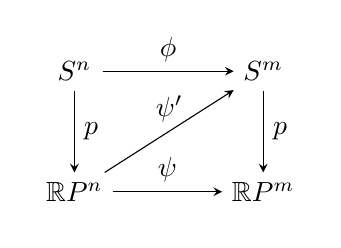
\begin{tikzpicture}
  \matrix (m) [matrix of math nodes,row sep=3em,column sep=4em,minimum width=2em] {
     S^n & S^m \\
     \mathbb{R}P^n & \mathbb{R}P^m \\};
  \path[-stealth]
    (m-1-1) edge node [right] {$p$} (m-2-1)
            edge  node [above] {$\phi$} (m-1-2)
    (m-2-1.east|-m-2-2) edge  node [above] {$\psi$} (m-2-2)
    (m-1-2) edge node [right] {$p$} (m-2-2)
            (m-2-1) edge  node [above]{$\psi'$} (m-1-2);
\end{tikzpicture}
\\
$\psi' \circ p$ and $\phi$ are both lifts of $\psi \circ p$ and both map $x\mapsto y$ so $\phi = \psi'\circ p$ by uniqueness. But then $\psi'(p(-x))=\psi'([x])=y=\phi(x)$, contradicting $\phi(-x)=-y$.
\end{proof}

\begin{definition}
Let $M^n$ be a closed oriented manifold with fundamental class $[M]\in H_n(M;\mathbb{Z})$. Let $[\alpha]\in H^a(M;\mathbb{Z})$ and $[\beta]\in H^{n-a+1}(M;\mathbb{Z})$ be torsion classes, i.e. $k[\alpha]=0,m[\beta]=0$ for some $k,m\in\mathbb{N}$. Then we can write $k\alpha=d\gamma$ for some $\gamma\in C^{a-1}(M,\mathbb{Z})$. We define $[\alpha]\vee[\beta]=\frac{1}{k}(\gamma\cup\beta)[M]\in\mathbb{Q}/\mathbb{Z}$.
\end{definition}
\begin{lemma}
$[\alpha]\vee[\beta]$ is well-defined and $[\beta]\vee[\alpha]=(-1)^{a(n-a+1)}[\alpha]\vee[\beta]$
\end{lemma}
\begin{proof}
Let $\gamma,\epsilon\in C^{a-1}(M,\mathbb{Z})$ such that $d\gamma=d\epsilon=k\alpha$.
$\frac{1}{k}(\gamma\cup\beta)[M]=\gamma(M\circ F_{e_0,...,e_a})$

$(k\alpha)\cup\beta=d(\alpha\cup\beta)+(-1)^{i+1}\alpha\cup d\beta=d\gamma\cup\beta=d\epsilon\cup\beta$
\end{proof}

\end{document}
